\documentclass[UKenglish]{beamer}


\usetheme[NoLogo, norsk]{MathDeptX}


\usepackage[utf8]{inputenx} % For æ, ø, å
\usepackage{babel}          % Automatic translations
\usepackage{csquotes}       % Quotation marks
\usepackage{microtype}      % Improved typography
\usepackage{amssymb}        % Mathematical symbols
\usepackage{mathtools}      % Mathematical symbols
\usepackage{amsmath}
\usepackage[absolute, overlay]{textpos} % Arbitrary placement
\setlength{\TPHorizModule}{\paperwidth} % Textpos units
\setlength{\TPVertModule}{\paperheight} % Textpos units
\usepackage{tikz}
\usepackage{tikz-cd}
\usetikzlibrary{overlay-beamer-styles}  % Overlay effects for TikZ
\usepackage{spectralsequences}
\usepackage{hyperref}


\author{Mika Bohinen}
\title{Rasjonale homotopigrupper av sfærer}


\begin{document}


\section{Oversikt}


% Use
%
%     \begin{frame}[allowframebreaks]{Title}
%
% if the TOC does not fit one frame.

\begin{frame}
\begin{figure}[]
    \centering
    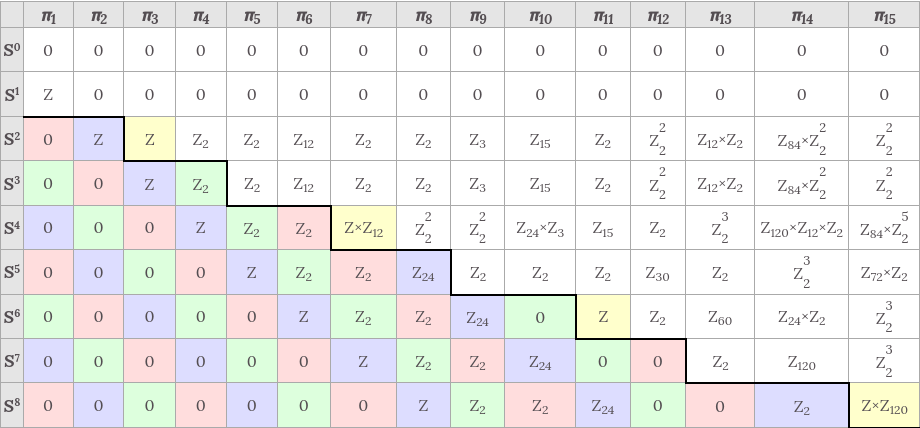
\includegraphics[width=0.8\textwidth]{figures/homotopigrupper.png}
    \caption{Hentet fra https://en.wikipedia.org/wiki/Homotopy\_groups\_of\_spheres}
    \label{fig:}
\end{figure}
\end{frame}

\begin{frame}{Det store resultatet}
   \begin{theorem}
      For \( n\in \mathbb{Z}^+ \) oddetall har vi at
      \begin{equation}
          \pi_k(S^n)\otimes \mathbb{Q} =
          \begin{cases}
              \mathbb{Q}, & k = n\\
              0, &  \text{ ellers.}
              
          \end{cases}
      \end{equation}
    og for \( n\in \mathbb{Z}^+ \) partall har vi at
    \begin{equation}
       \pi_k(S^n)\otimes \mathbb{Q} =
       \begin{cases}
           \mathbb{Q}, & k=n, 2n-1\\
           0, & \text{ ellers.}
           
       \end{cases}
    \end{equation}
  \end{theorem}
\end{frame}
\begin{frame}{Innholdsfortegnelse}
    \tableofcontents
\end{frame}


\section{Bakgrunnsstoff}

\subsection{Homotopigrupper}


\begin{frame}{Homotopigrupper}
    \begin{definition}[Veirom]
       Gitt en punktet rom \( (X, x_0) \) definerer vi \( PX \) som
       alle kontinuerlige avbildninger \( \alpha:[0,1]\rightarrow X \)
       slik at \( \alpha(0)=x_0 \). Løkkerommet \( \Omega X \) er
       underrommet av \( PX \) slik at \( \alpha(1)=x_0 \).
    \end{definition}
    \begin{definition}[]
    Gitt et punktet rom \( (X, x_0) \), la \( \pi_0(X, x_0) \) 
    være veikomponentene til rommet. Definer de resterende homotopigruppene
    induktivt ved
    \begin{equation}
        \pi_{n+1}(X, x_0) = \pi_n(\Omega X, \bar{x}_0)
    \end{equation}
    hvor \( \bar{x}_0 \) 
    er den konstante veien ved \( x_0 \). Komposisjon fungerer
    som gruppeoperasjon.
    \end{definition}
    \iffalse
    Intuitivt tenker vi på elementer i homotopigruppene som avbildninger
    fra sfærer til rommet. Vi kan for eksempel tenke på fundamentalgruppen
    \( \pi_1(X, p) \) som forskjellige måter å strekke ut en lukket strikk i
    rommet.
    \fi
    
\end{frame}


\iffalse
\subsection{Serrefibrasjon}
\begin{frame}[c]{Serrefibrasjon}
   \begin{definition}[]
    En avbildning \( p:E\rightarrow B \) kalles en serrefibrasjon hvis
    \( p \) har homotopiløftingsegenskapen for alle CW-komplekser.
   \end{definition}
   \pause
   \begin{proposition}
       Gitt et punktet rom \( (X, x_0) \) så er \( \chi:PX\rightarrow X \) 
       definert ved \( \chi(\alpha)=\alpha(1) \) en serrefibrasjon.
   \end{proposition}
\end{frame}
\fi


\subsection{Eilenberg-Maclane rom}

\begin{frame}[t]
    \frametitle{Eilenberg-Maclane rom}
   \begin{definition}
      Gitt en gruppe \( G \) og \( n\in \mathbb{Z}^+ \) så sier vi at
      et rom \( X \) er av type \( K(G, n) \) hvis den \( n \)-te 
      homotopigruppen er isomorf med \( G \) og ellers triviell.
   \end{definition} 
    \pause
    \begin{proposition}
       For hver abelske gruppe \( G \) og \( n\geq 2 \) har vi en
       serrefibrasjon
       \begin{equation}
           \begin{tikzcd}
               {K(G,n-1)} & {*} & {*} & {K(G, n)} & {K(G,n)}
             \arrow[from=1-1, to=1-2]
             \arrow[from=1-2, to=1-3]
           \end{tikzcd}
       \end{equation}
    \end{proposition}
    \pause
    \begin{proof}
       Bruk veiromfibrasjonen på \( K(G, n) \). 
    \end{proof}
\end{frame}

\subsection{Rasjonal homotopiekvivalens}
\begin{frame}{Rasjonal homotopiekvivalens}
   \begin{definition}
      La \( f:X\rightarrow Y \) være en avbildning. Vi sier at \( f \) 
      er en rasjonal homotopiekvivalens hvis den induserte avbildningen
      \( \pi_*(f)\otimes\mathbb{Q}:\pi_*(X)\otimes\mathbb{Q}\rightarrow \pi_*(Y)\otimes\mathbb{Q} \) 
      er en isomorfi.
   \end{definition} 
    \pause
    \begin{theorem}[]
        En avbildning \( f:X\rightarrow Y \) er en rasjonal homotopiekvivalens
        hvis og bare hvis 
        den induserte avbildningen \( f^*:H^*(Y;\mathbb{Q})\rightarrow H^*(X;\mathbb{Q}) \) 
        er en isomorfi.
    \end{theorem}
    \pause
\end{frame}


\section{Spektralfølger}
\SectionPage


\begin{frame}{Spektralfølger}
    \begin{figure}[]
        \centering
        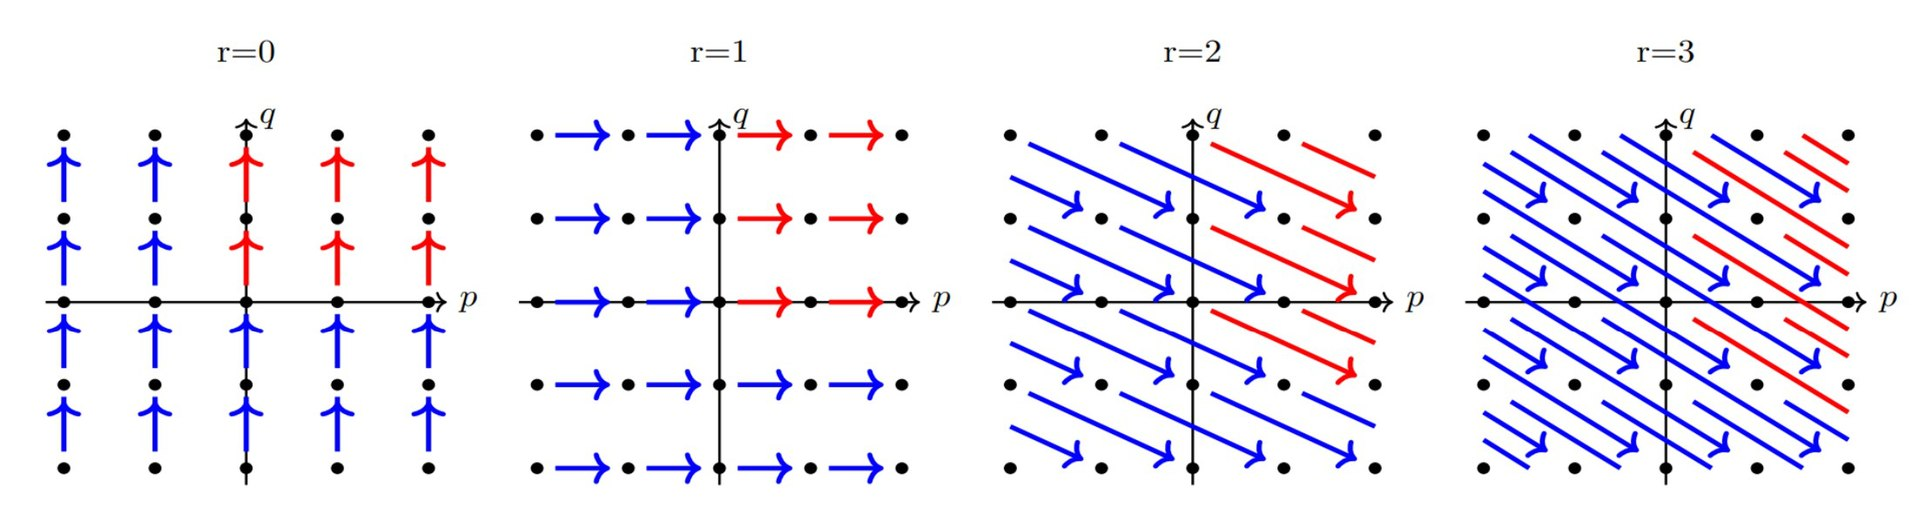
\includegraphics[width=\textwidth]{figures/specseq.jpg}
        \caption{Av L.penguu, hentet fra \href{https://en.wikipedia.org/wiki/Spectral_sequences}{https://en.wikipedia.org/wiki/Spectral\_sequences} distribuert under \href{https://creativecommons.org/licenses/by-sa/4.0/}{CC BY-SA 4.0}}
        \label{fig:}
    \end{figure}
\end{frame}

\begin{frame}
   \begin{definition}[Bigradert abelsk gruppe]
      En bigradert abelsk gruppe \( E_r = E_r^{*,*} \) er en dobbelindeksert 
      direkte sum av abelske grupper,
      \begin{equation}
          E_r^{*,*} = \bigoplus_{p,q\in\mathbb{Z}} E_r^{p,q}
      \end{equation}
        hvor \( (p, q) \) kalles bigraden til en gruppe i summen.
   \end{definition} 
    \pause

    \begin{definition}[Spektralfølge]
        En spektralfølge \( E \) er en samling av bigraderte
        abelske grupper \(\{E_r\}_{r\in\mathbb{Z}^+}  \) og endomorfier 
        \( \{d_r:E_r\rightarrow E_r\}_{r\in\mathbb{Z}^+} \) i bigrad \( (r, r-1) \) slik at
        \( d_r\circ d_r =0 \) og \( E_{r+1} \) er kohomologien til
        \( E_r \).
    \end{definition}
\end{frame}


\subsection{Konvergens}

\begin{frame}[c]{Konvergens av spektralfølger}
    \begin{itemize}
        \item Skjer ofte at \( E_{r+k}\cong E_r \) for alle \( k\in\mathbb{Z}^+ \) 
        \pause
        \item I dette tilfellet lar vi \( E_\infty \) stå for denne
        grensen
        \pause
    \item Gitt en gradert abelsk gruppe \( A^* \) så sier vi at spektralfølgen 
        \( E \) konverger mot \( A^* \) hvis for alle \( n\in\mathbb{Z} \) 
        \begin{equation}
            A^n \cong \bigoplus_{p+q =n} E_\infty^{p,q}.
        \end{equation}
    \end{itemize}
\end{frame}

\iffalse
\subsection{Spektralfølge av algebraer}

\begin{frame}[c]
    \frametitle{Spektralfølge av algebraer}
   \begin{definition}[]
      En spektralfølge av algebraer er en spektralfølge \( E \) slik at
      hver side \( (E_r, d_r) \) i følgen er en differensialbigradert
      algebra. Det vil si at for alle \( r\in \mathbb{Z}^+ \) så er
      \( d_r \) en antiderivasjon og i tillegg er det et produkt
      \( E_r\otimes E_r\rightarrow E_r \) slik at produktet i \( E_{r+1} \) 
      sammenfaller med det induserte produkte når vi tar kohomologien
      av \( E_r \).
   \end{definition} 
    \pause
    Konvergens for spektralfølger av algebraer er definert på nesten samme måte
    med et ekstra krav om at det induserte produktet i \( E_\infty \) 
    må sammenfalle med produktet i \( A^* \).
\end{frame}
\fi


\subsection{Leray-Serre spektralfølgen}

\begin{frame}[c]
    \frametitle{Leray-Serre spektralfølgen}
    \begin{theorem}[]
       La \( R \) være en kommutativ ring med enhet og 
       \( F\rightarrow E \rightarrow B \) en serrefibrasjon
       hvor \( B \) er veisammenhengende. Det eksisterer da en førstekvadrant
       spektralfølge av algebraer \( E \) som konverger mot \( H^*(E;R) \)
       som en algebra og med \( E_2^{p,q}\cong H^p(B; H^q(F;R)) \).

    \end{theorem} 
\end{frame}

\section{Rasjonal kohomologi algebra av \( K(\mathbb{Z}, n) \)}
\SectionPage


\begin{frame}[allowframebreaks]
    \begin{theorem}[]
       For \( n\in \mathbb{Z}^+ \) partall har vi at
       \begin{equation}
           H^*(K(\mathbb{Z}, n);\mathbb{Q})\cong \mathbb{Q}[x]
       \end{equation}
        hvor \( |x|=n \) mens for \( n \in \mathbb{Z}^+ \) oddetall har
        vi at
        \begin{equation}
            H^*(K(\mathbb{Z}, n);\mathbb{Q})\cong \Lambda_\mathbb{Q}(x)
        \end{equation}
        med \( |x|=n \).
    \end{theorem}    
    \begin{proof}
        Gjøres ved induksjon på \( n \). For \( n=1 \) vet vi at
        \( K(\mathbb{Z}, 1)\simeq S^1 \) og her kan man komme fram til
        resultatet via for eksempel de Rham teori. Anta at \( n> 1 \) er
        partall slik at \( n-1 \) er oddetall. Vi kan nå bruke
        Leray-Serre spektralfølgen på fibrasjonen
        \begin{equation}
            K(\mathbb{Z}, n-1)\rightarrow *\rightarrow K(\mathbb{Z}, n)
        \end{equation}
        Her er et eksempel med \( n=4 \). \\
       
        Vi ser altså at \( H^*(K(\mathbb{Z}, n); \mathbb{Q})\cong \mathbb{Q}[x] \)
        med \( |x|=n \).
    \end{proof}
\end{frame}

\begin{frame}[c]
       \begin{figure}
           \centering
        \begin{sseqpage}[classes = {draw = none}, cohomological Serre grading]
          \class["\mathbb{Q}"](0, 0)
          \class["\mathbb{Q}_y"](0, 3)
          \class["\mathbb{Q}_x"](4, 0)
          \class["\mathbb{Q}_{xy}"](4, 3)
          \class["\mathbb{Q}_{x^2}"](8, 0)
          \class["\mathbb{Q}_{x^2 y}"](8, 3)

          \d4(0, 3) 
          \d4(4, 3)
          \d4(8, 3)
        \end{sseqpage}
       \end{figure} 
\end{frame}


\section{Beviset}
\SectionPage
\begin{frame}[c]
    \frametitle{Oddetallsfærene}
   \begin{theorem}[]
       For \( n\in \mathbb{Z}^+ \) oddetall har vi at
       \begin{equation}
           \pi_k(S^n)\otimes \mathbb{Q} =
           \begin{cases}
               \mathbb{Q}, &\text{ hvis } k = n\\
              0, &\text{ ellers.} 
           \end{cases}
       \end{equation}
   \end{theorem} 
\end{frame}

\begin{frame}[t, allowframebreaks]
   \begin{proof}
      Vi ønsker å finne en isomorfi \( f^*:H^*(K(\mathbb{Z}, n);\mathbb{Q})
      \rightarrow H^*(S^n; \mathbb{Q})\) slik at vi kan bruke teoremet om
      rasjonale homotopiekvivalens. La derfor \( f:S^n \rightarrow K(\mathbb{Z}, n)
    \) være en representant for generatoren av \( \pi_n(K(\mathbb{Z}, n)) \).
    Dette betyr at \( f_*\otimes\text{id}:\pi_n(S^n)\otimes\mathbb{Q}
    \rightarrow \pi_n(K(\mathbb{Z}, n))\otimes \mathbb{Q}\) er en
    isomorfi. I tillegg har vi et kommutativt diagram.\\

    Vi ser altså at \( f^*:H^n(K(\mathbb{Z}, n);\mathbb{Q})\rightarrow
    H^n(S^n;\mathbb{Q})\) er en isomorfi. Dermed må \( f^*:H^*(K(\mathbb{Z}, n);\mathbb{Q})\rightarrow H^*(S^n;\mathbb{Q}) \) være en isomorfi.

   \end{proof} 
\end{frame}

\begin{frame}[]
    
    \begin{figure}[]
        \centering
        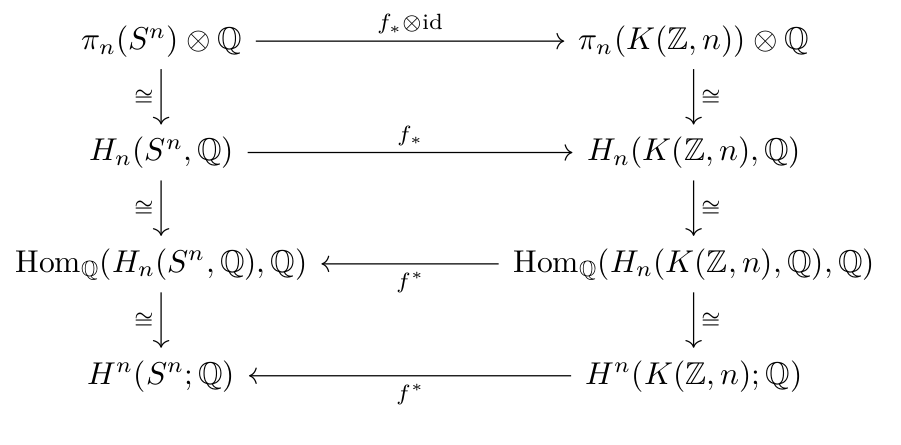
\includegraphics[width=\textwidth]{figures/commutative.png}
    \end{figure}
\end{frame}


\begin{frame}
\begin{figure}[]
    \centering
    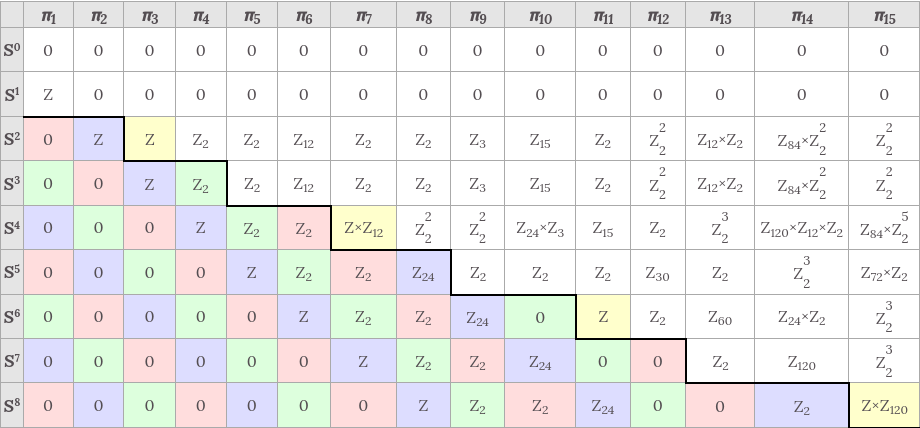
\includegraphics[width=0.8\textwidth]{figures/homotopigrupper.png}
    \label{fig:}
\end{figure}
\end{frame}
\end{document}
